\documentclass[10pt,twocolumn]{article}

% Följande rad ska göra det möjligt att använda svenska bokstäver, som å, ä, ö. Kravet är 
% då att filen sparas i UTF-8-format. Om detta inte fungerar för dig, så kan du alltid 
% använda dig av {\aa} för å, \"a för ä och \"o för ö.
\usepackage[utf8]{inputenc}

\usepackage[swedish]{babel}

% Följande väljer typsnitt som är kloner av Times New Roman, Helvetica och lämpliga till
% dem anpassade matematiktypsnitt.
\usepackage{newtxtext}
\usepackage{newtxmath}

%  Programkod
\usepackage{listings}
\usepackage{color} %red, green, blue, yellow, cyan, magenta, black, white
\definecolor{mygreen}{RGB}{28,172,0} % color values Red, Green, Blue
\definecolor{mylilas}{RGB}{170,55,241}
\definecolor{gray}{RGB}{88,88,88}
\lstset{language=Matlab,%
    %basicstyle=\color{red},
    breaklines=true,%
    morekeywords={matlab2tikz},
    keywordstyle=\color{blue},%
    morekeywords=[2]{1}, keywordstyle=[2]{\color{black}},
    identifierstyle=\color{black},%
    stringstyle=\color{mylilas},
    commentstyle=\color{mygreen},%
    showstringspaces=false,%without this there will be a symbol in the places where there is a space
    numbers=left,%
    numberstyle={\tiny \color{gray}},% size of the numbers
    numbersep=5pt, % this defines how far the numbers are from the text
    emph=[1]{for,end,break},emphstyle=[1]\color{red}, %some words to emphasise
    %emph=[2]{word1,word2}, emphstyle=[2]{style},    
}

% Figurer
\usepackage{graphicx}
\graphicspath{{img/}}
\usepackage{float}

% Citat
\usepackage{dirtytalk}

\raggedbottom
\sloppy

\title{Laborationsrapport i TSKS10 \emph{Signaler, Information och Kommunikation}}

\author{Matti Lundgren \\ matlu703, xxyyzz-ååää }

\date{19 maj, 2017}

\begin{document}

\maketitle

\clearpage

\section{Inledning}

Laborationen går ut på att demodulera en smalbandig, I/Q-modulerad signal som består av hörbart ljud. Det är givet att den utsända signalen har utseendet $x(t)=x_I(t)cos(2\pi f_ct)-x_Q(t)sin(2\pi f_ct)+w(t)+z(t)$ där $w(t) = 0.001(cos(2\pi f_1t) + cos(2\pi f_2t))$ och $z(t)$ är en summa av signaler som sänds på andra bärfrekvenser. 

På grund av ekoeffekter blir den mottagna signalen $y(t)=x(t-\tau_1)+0,9x(t-\tau_2)$. Termerna är förskjutna med $\tau_1$ sekunder då det är tiden det tar för signalen att nå mottagaren. Den andra termen är resultatet av ekot som orsakar en energiförlust på 10\% och som bidrar med en tidsförskjutning på $\tau_2$ - $\tau_1$ sekunder.

Annan relevant information given av laborationshanledningen listas nedan:
\begin{itemize}
\item Bärfrekvensen $f_c$ är någon av följande frekvenser: 18, 37, 56, 75, 94, 113, 132, 151 kHz.
\item $f_1$ och $f_2$ är multiplar av 1 Hz och överlappar inte med någon av de burna signalerna.
\item $\tau_2>\tau_1$, $\tau_2-\tau_1<500$ ms och $\tau_2-\tau_1$ är en multipel av 1 ms.
\item Då signalerna ska bestå av hörbart ljud sätts deras intressanta bandbredd till $B=20$ kHz.
\end{itemize}

\section{Metod}

För att genomföra laborationen användes, utöver laborationshandledningen, kursboken \textit{Signals, Information and Communications} (utkast 14273) och Matlab. Programkoden bifogas på sida 4 och de plottade figurerna på sida 3.

$y(t)$s amplitudspektrum plottas i figur 1. Ur spektrumet identiferas tre möjliga bärfrekvenser; 56, 94 och 151 kHz. De burna signalerna benämns hädanefter som $y_1(t)$, $y_2(t)$ respektive $y_3(t)$. Signalerna erhålls genom att bandpassfiltrera $y(t)$ runt respektive bärfrekvens med bandbredden $B$. De plottas i figur 2 där $y_1(t)$ ser ut att vara nyttosignalen.

$w(t)$ ser ut att existera runt 46,5 kHz, därför plottas $y(t)$s amplitudspektrum runt denna frekvens, se figur 3. Då det är känt att $f_1$ och $f_2$ är multiplar av 1 Hz går det att dra slutsatsen att $f_1=46500$ Hz och att $f_2=46501$ Hz.

För att ta reda på tidsfördröjningen $\tau_2-\tau_1$ används tidsestimering med korskorrelation som beskrivs av kursbokens fjärde kapitel. $y(t)$ korskorrelerat med sig själv benämns som $r(\tau)$ och plottas i figur 4. Tidsfördröjningen ges av det $\tau$ som bortsett från den första toppen ger $r(\tau)$ sitt största värde. Med hjälp av figur 4 identifieras det sökta $\tau$ till att vara 430 ms vilket är troligt då det är känt att $\tau_2-\tau_1 < 500$ ms och att differensen är en multipel av 1 ms. Slutsatsen blir att $\tau_0$ är tidsfördröjningen orsakat av ekot, det vill säga $\tau_0=\tau_2-\tau_1=430$ ms.

Ekot annulleras med hjälp av ekvationen $\hat{y}(t)=y(t) - 0,9\hat{y}(t-\tau_0)$ för $t > \tau_0$. Ekvationen för $\hat{y}(t)$ härleds ur ekvationen för $x(t)$ genom att bortse från tidsfördröjningen $\tau_1$ som orsakas av avståndet mellan sändare och mottagare. Notera att $\hat{y}(t)$ är den ekofria signalen och att $y(t)$ är fri från eko då $t < \tau_0$. Då den sökta signalen tros vara $y_1(t)$ behandlas endast den. 

Nu återstår demoduleringen. Ur kursbokens andra kapitel framgår det att $\hat{y}_I(t)=H^{LP}_{B/2}\{2\hat{y}(t)cos(2\pi f_{c}t+\delta)\}$ och att $\hat{y}_Q(t)=H^{LP}_{B/2}\{-2\hat{y}(t)sin(2\pi f_{c}t+\delta)\}$. Då $\hat{y}(t)$ i det här fallet är en ekofri variant av $y_1(t)$ är bärfrekvensen $f_c=56$ kHz. Signalen lågpassfiltreras med lägre bandbredd än $B/2$ för att minimera oönskat ljud. En fasvridning kan behöva kompenseras för, den representeras av $\delta$ i demoduleringsekvationerna. Efter prövning sätts $\delta=1.1$ radianer vilket verkar minimera de talade ordspråkens överlapp.

\section{Resultat}

Den sökta informationen är:
\begin{itemize}
\item Bärfrekvensen för nyttosignalen är $f_c=56$ kHz.
\item Sinusoidernas frekvenser i $w(t)$ är $f_1=46500$ Hz och $f_2=46501$ Hz.
\item Ekots bidrag till tidsfördröjningen är $\tau_2-\tau_1=430$ ms.
\item Ordspråket i $x_I(t)$ är \say{Inget ont som inte har något gott med sig}.
\item Ordspråket i $x_Q(t)$ är \say{Även den mest skröpliga mussla kan innehålla en pärla}.
\end{itemize}

\clearpage

\section*{Figurer}

\begin{figure}[H]
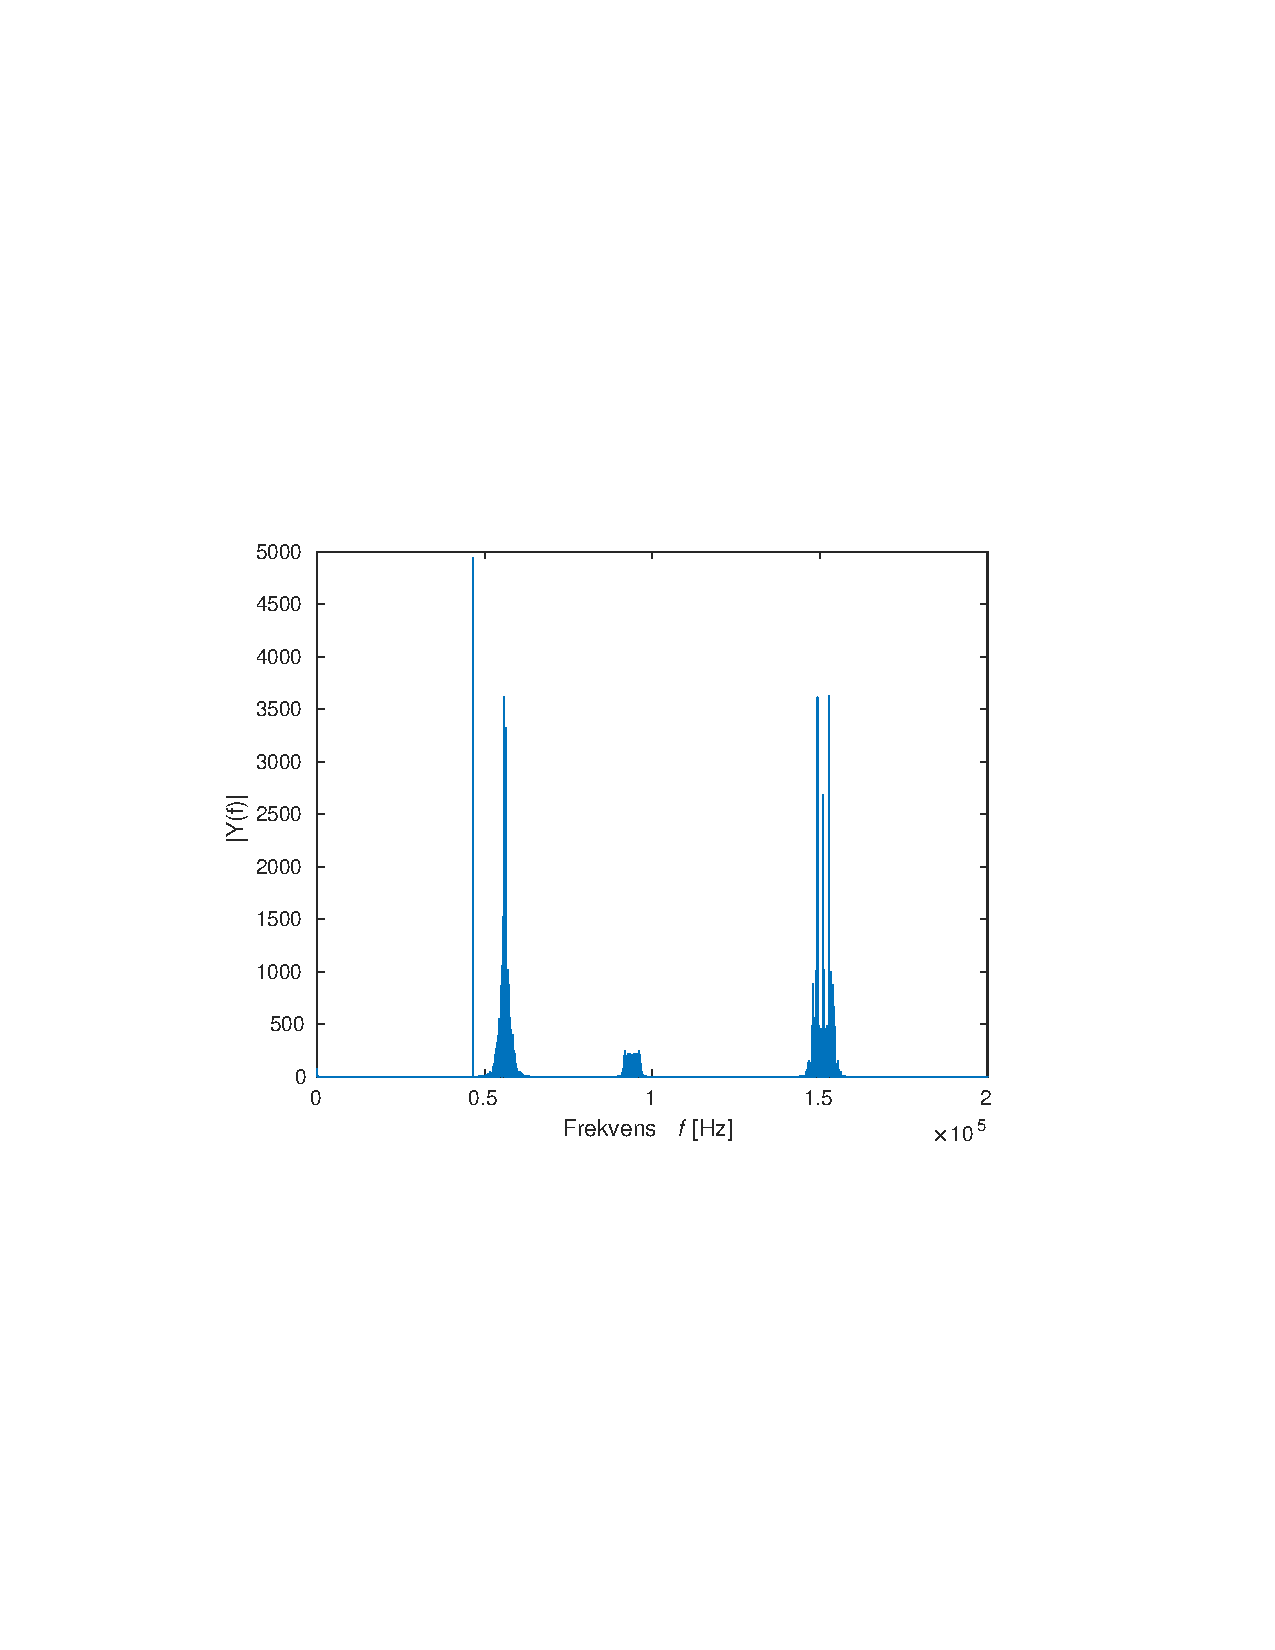
\includegraphics[trim={3.8cm 8cm 4.8cm 9cm},clip,width=8cm]{Y.pdf}
\caption{Amplitudspektrum för $y(t)$}
\end{figure}

\begin{figure}[H]
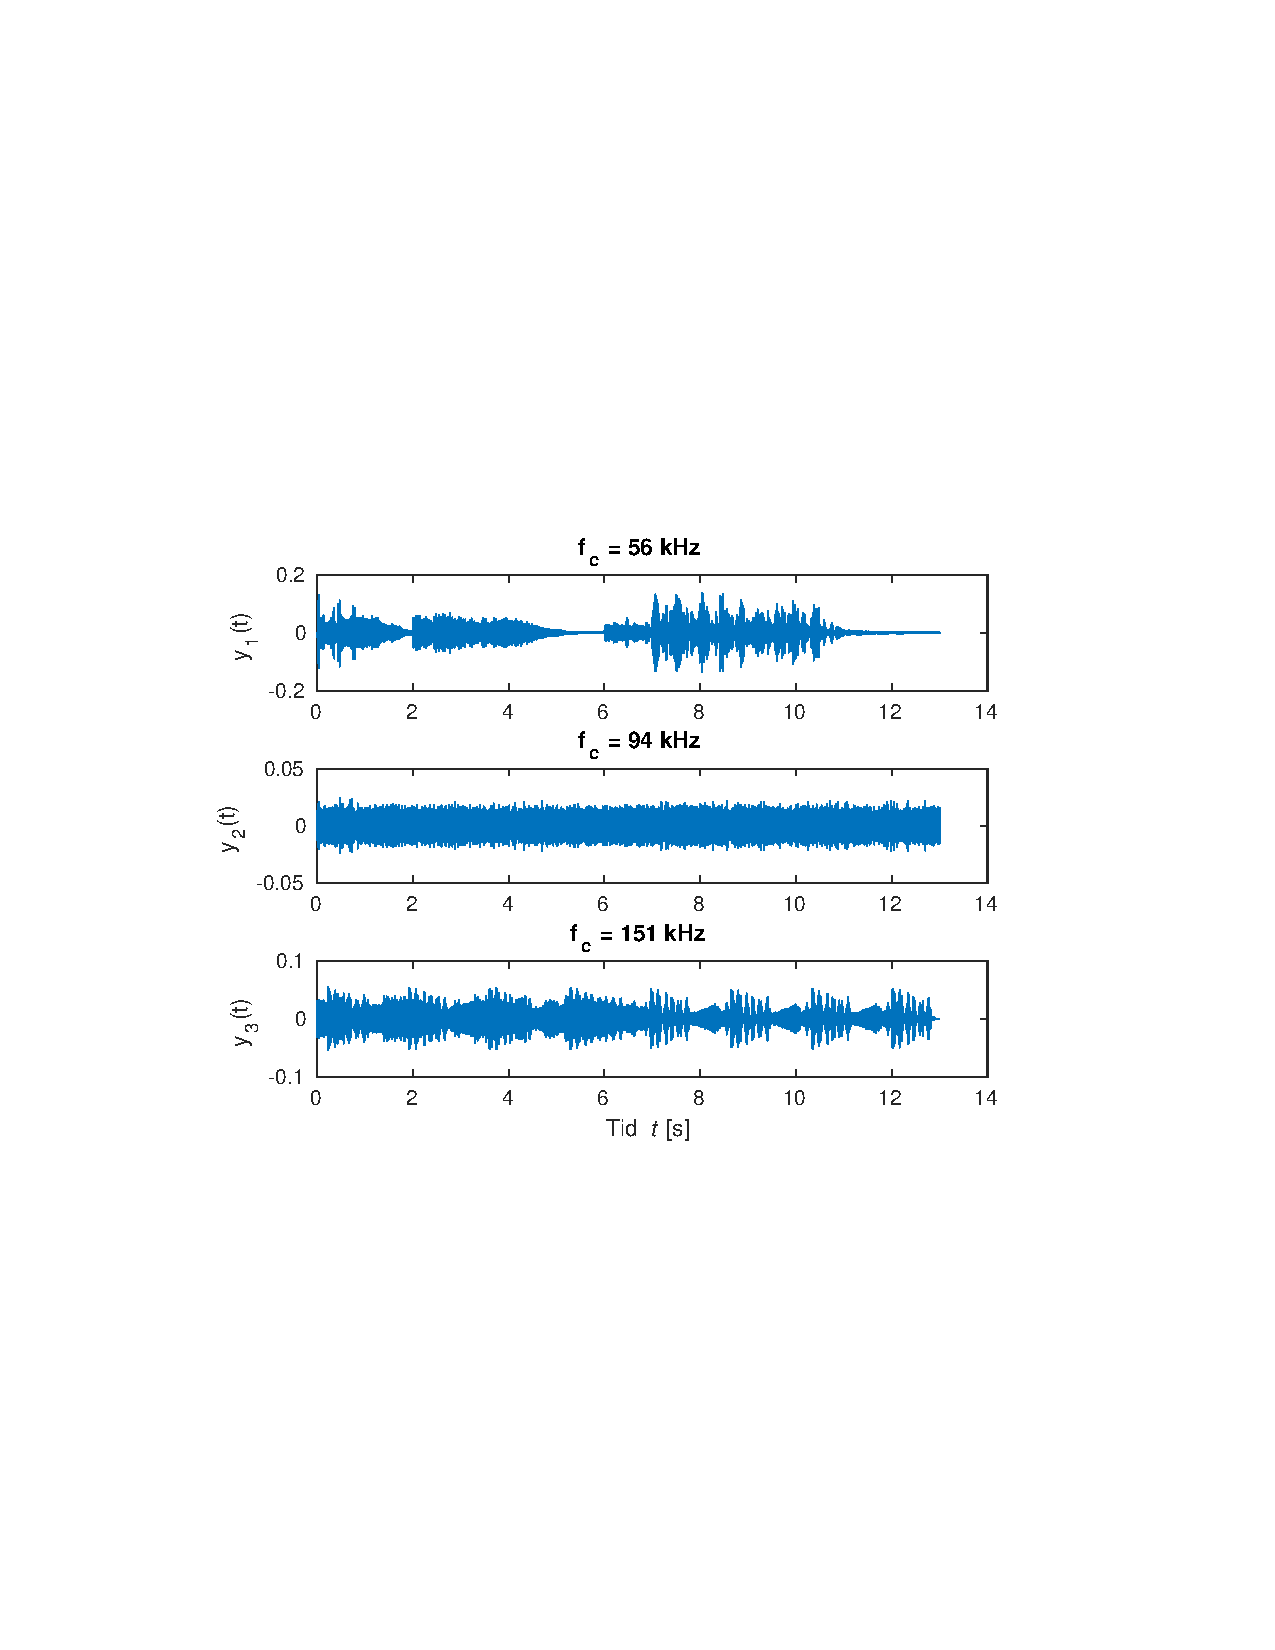
\includegraphics[trim={3.8cm 8cm 4.8cm 9cm},clip,width=8cm]{carried_signals.pdf}
\caption{De tre identifierade delsignalerna}
\end{figure}
\section*{ }
\begin{figure}[H]
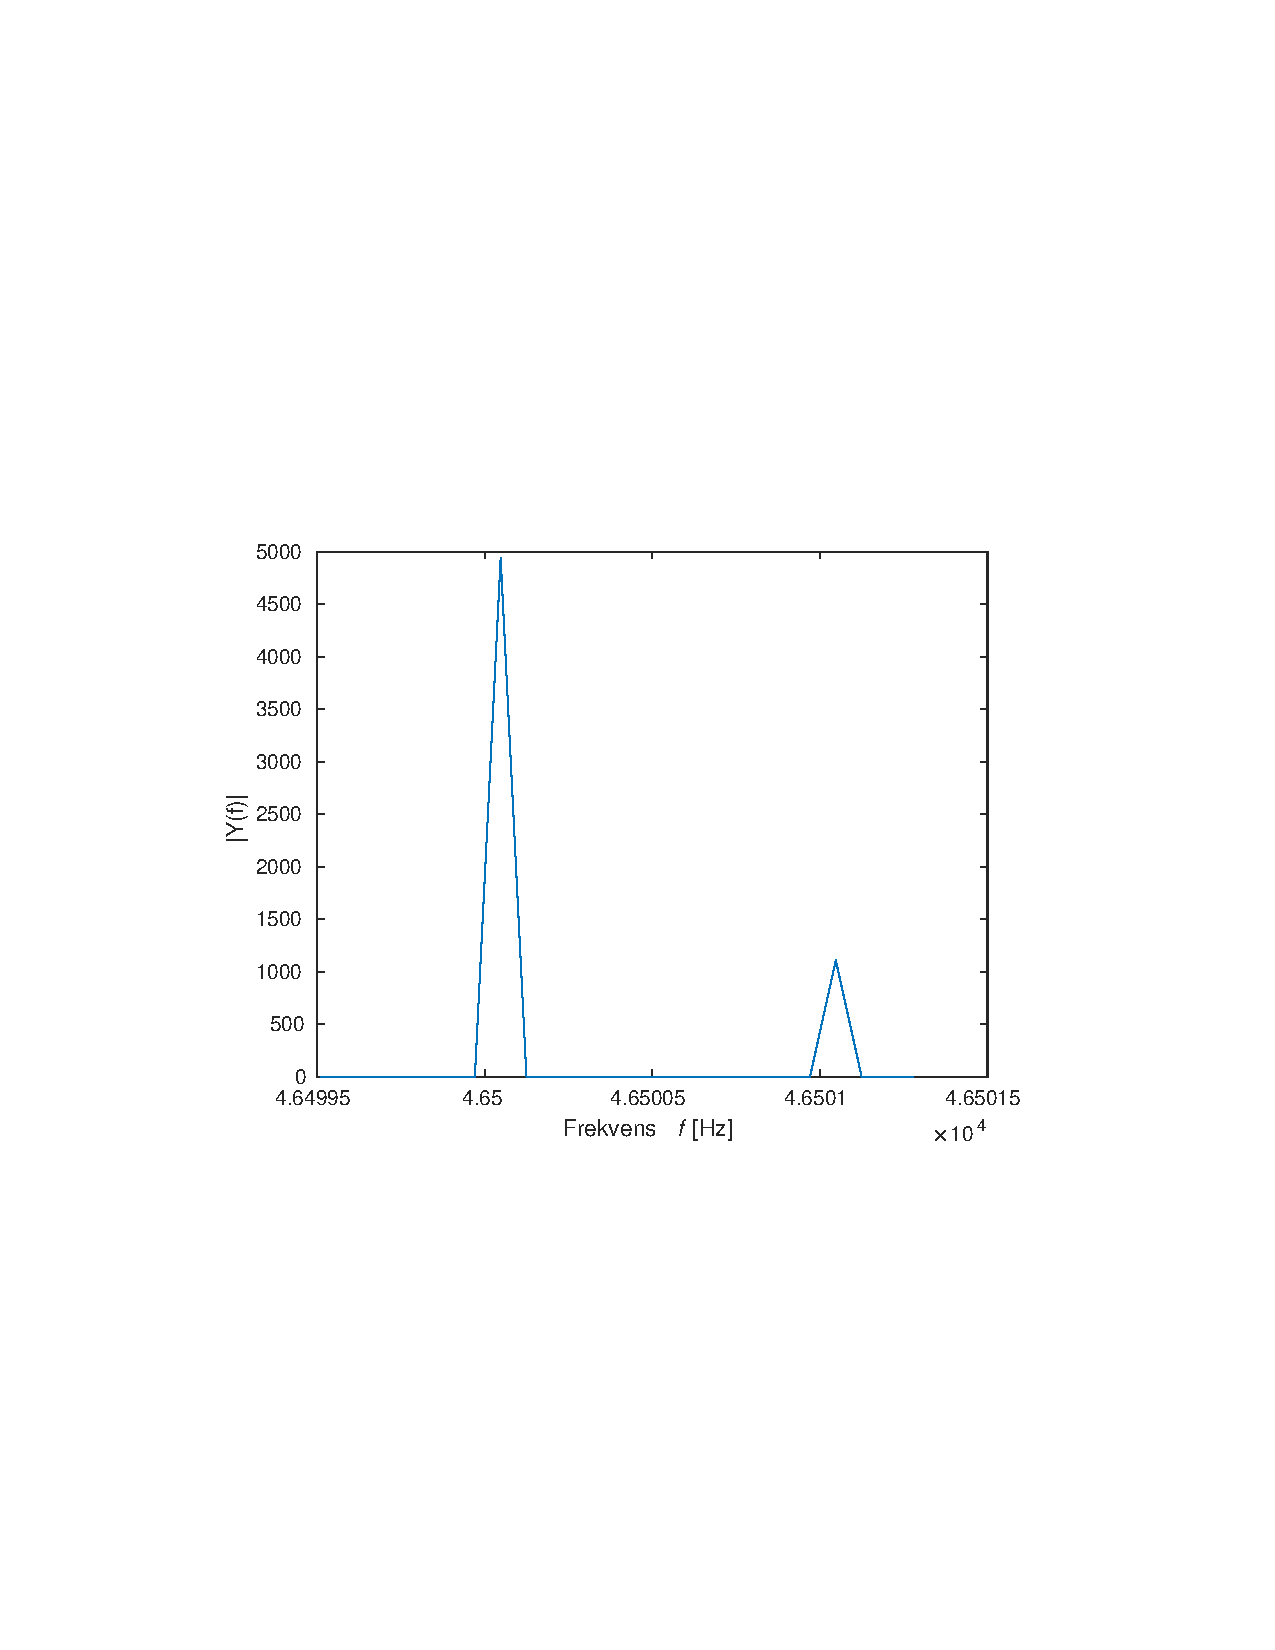
\includegraphics[trim={3.8cm 8cm 4.8cm 9cm},clip,width=8cm]{Y_46_5kHz.pdf}
\caption{Amplitudspektrum för $y(t)$ runt 46.5 kHz}
\end{figure}

\begin{figure}[H]
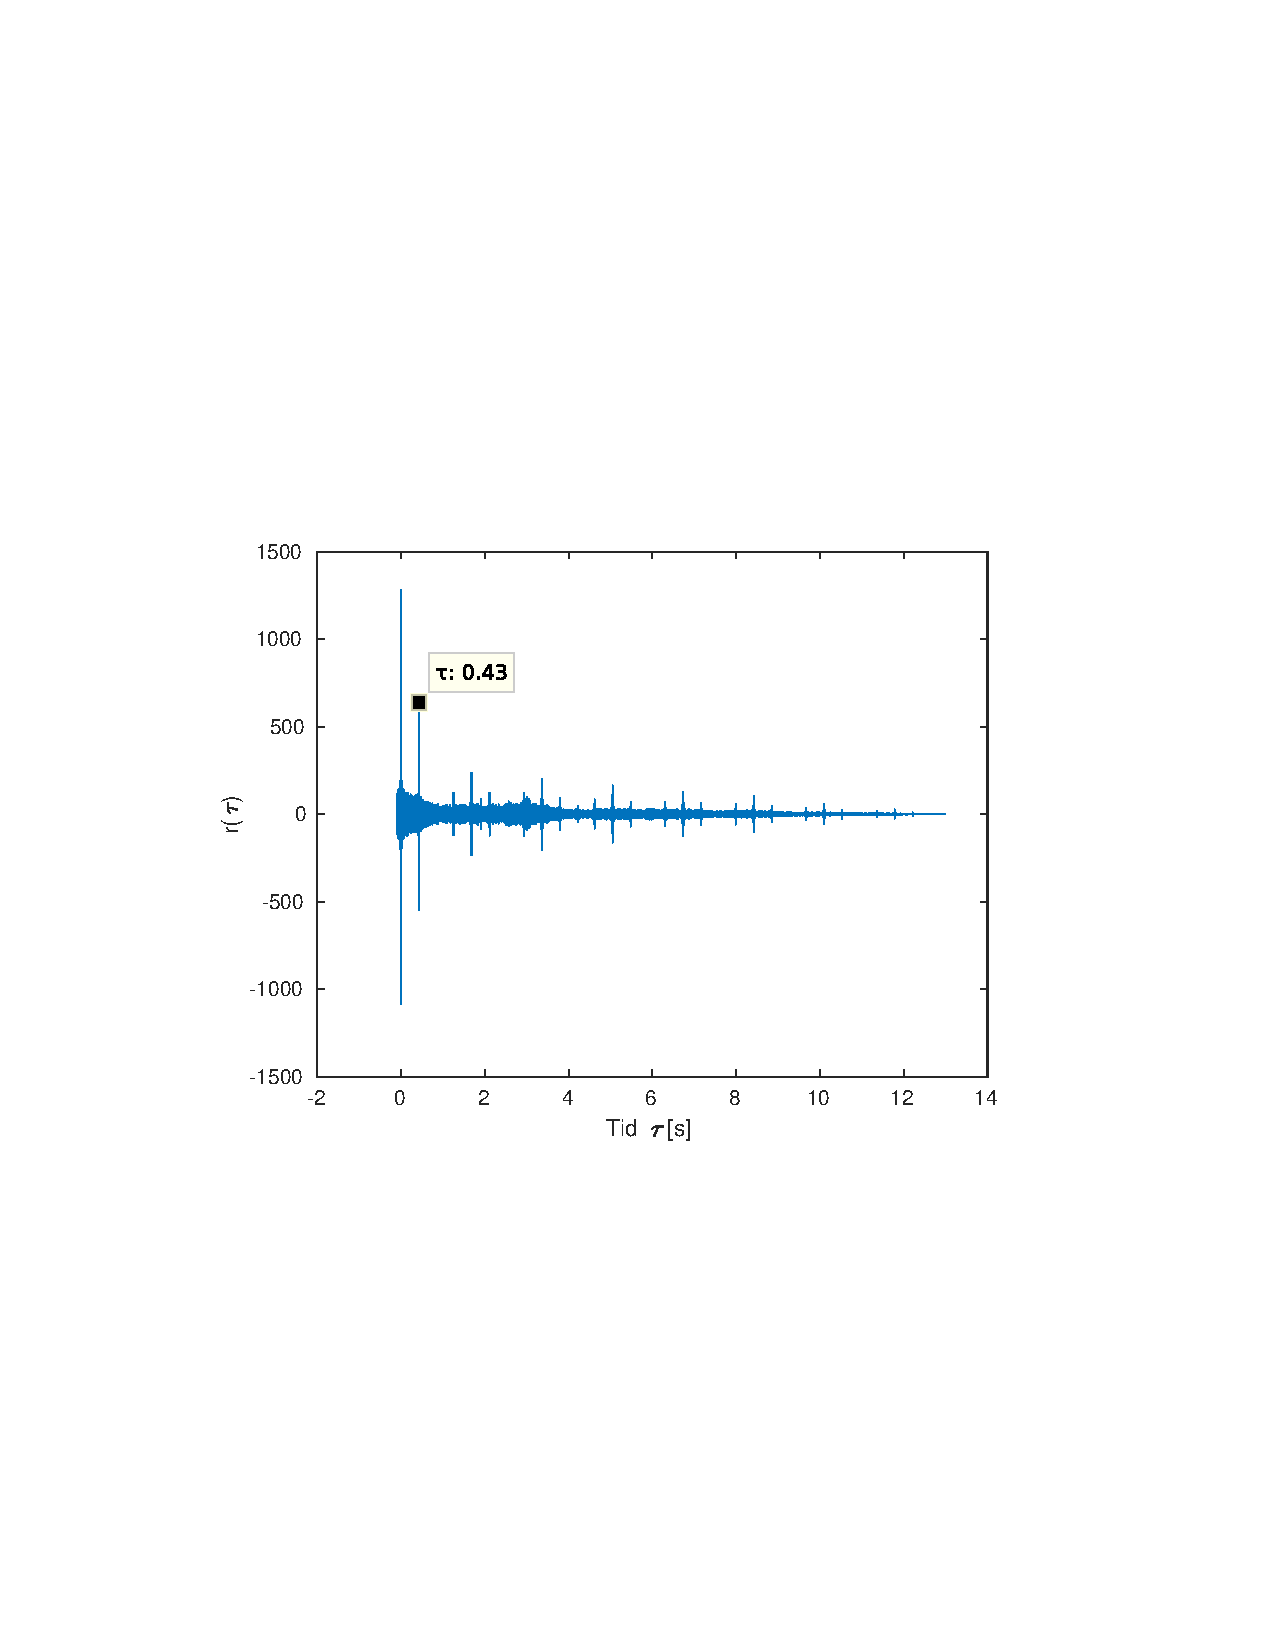
\includegraphics[trim={3.8cm 8cm 4.8cm 9cm},clip,width=8cm]{xcorr.pdf}
\caption{$y(t)$ korskorrelerat med sig själv med betoning på $\tau$ för den högsta sidotoppen}
\end{figure}

\clearpage

\section*{Matlab-kod}
\small
\texttt{\lstinputlisting[language=Matlab,breaklines=true]{tsks10.m}}
\end{document}
